\documentclass{article}

\usepackage[colorlinks,linkcolor=red]{hyperref} %链接
\usepackage[round]{natbib} %参考文献
\usepackage{newtxtext,newtxmath}
\usepackage{graphicx}
\usepackage{caption}
\usepackage[UTF8]{ctex}

\author{Gil Levi,Tal Hassner}
\title{基于卷积神经网络的年龄性别分类研究}

\begin{document}
\maketitle
\begin{abstract}
随着社交媒体与社交平台的兴起,自动化的年龄与性别分类已经与越来越多的应用相关联。
尽管如此,现存的理论方法在真实世界图像任务上依然十分的缺乏,特别是与最近针对面部识别领域所取得的巨大进步相比。
在文中,我们使用深度卷积网络来学习,使之可以在这些任务上获得巨大的提升。
为此我们提出了一种简单的神经网络架构,即使在学习数量级数目有限的情况下也可以使用。
我们根据最近的年龄和性别的Adience基准评估方法,将其标记为显著优于目前最佳算法的方法。
\end{abstract}

\section{导言}
年龄和性别在社会互动中发挥着重要作用。
语言在男性或女性之间有着不同的称呼和语法规则,这一点年轻人与老年人之间更甚。
尽管这些属性在我们的日常生活中发挥了基本作用,但是从面部图像中准确可靠地自动估计它们的能力仍然远远不能满足商业应用的需求。
在考虑最近在面部识别相关任务中对超人类能力的主张时,这尤其令人困惑。\\

从面部图像估计或分类这些属性的过去方法依赖于面部特征维度或“定制”面部描述符的差异。
大多数人采用了专为年龄或性别评估任务而设计的分类方案,包括[1]和其他方法。
这些过去的方法很少被设计用于应对无约束成像条件的许多挑战。
此外,这些系统采用的机器学习方法没有充分利用通过互联网提供的大量图像示例和数据来提高分类能力。\\

在本文中,我们试图缩小自动人脸识别能力与年龄和性别估计方法之间的差距。
为此,我们遵循最近的人脸识别系统所规定的成功例子:过去几年描述的人脸识别技术已经表明,使用深度卷积神经网络(CNN)可以取得巨大进步。
我们通过简单的网络架构证明了这样的确可以获得很大的收益,该架构是通过考虑现有面部数据集中准确的年龄和性别标签的相当有限的可用性而设计的。\\

我们以新发布的Adience基准测试我们的网络,用于未过滤面部图像的年龄和性别分类。
我们表明,尽管Adience上的图像非常具有挑战性,并且我们的网络设计非常简单,但我们的方法在很大程度上优于现有技术水平。
虽然这些结果为基于深度学习的方法提供了显着的基础线路,但它们也为更精细的系统设计留下了改进空间,在无约束的设置中准确估计年龄和性别的问题上,比如由Adience图像反射的问题仍未解决。
为了为开发更有效的未来方法提供立足点,我们公开了经过培训的模型和分类系统,更多的信息,请查看:\url{http://www.openu.ac.il/home/hassner/projects/cnn_agegender}\\

\section{相关工作}
在描述所提出的方法之前,我们简要回顾一下年龄和性别分类的相关方法,并对深度卷积网络做一个简单介绍。
\subsection{年龄和性别分类}
\textbf{年龄分类}
近年来,从面部图像中自动提取年龄相关属性的问题受到越来越多的关注,并且已经提出了许多方法。这些方法的详细调查可以在[2]和最近的[3]中找到。
我们注意到,尽管我们关注的是年龄组分类而不是精确的年龄估计(即年龄回归),但调查结果显示任一任务都可以使用这种设计方法。\\

早期的年龄估计方法是基于计算不同面部特征测量值之间的比率。一些面部特征(例如,眼睛,鼻子,嘴巴,下巴等)被局部化并且测量它们的尺寸和距离,就会计算它们之间的比率并用于根据人工制定的规则将面部分成不同的年龄类别。
最近,[4]使用类似的方法来模拟测试18岁以下受试者的年龄。由于这些方法需要准确定位面部特征,但这本身就是一个具有挑战性的问题,因此它们不适合人们在社交平台上找到的无规则图像。\\

在另一项工作中,有一些方法将衰老过程表示为子空间或流形。这些方法的缺点是它们需要输入图像近似规则和良好对齐。
因此,这些方法仅在受限的近前图像数据集(例如UIUC-IFP-Y [12,19],FG-NET [30]和MORPH [43])有用。
同样,这种方法不适合于不受约束的图像。\\

与上述不同的是使用局部特征来表示面部图像的方法。用高斯混合模型(GMM)来表示面部贴片的分布。
在[5]中,GMM再次用于表示局部面部测量的分布,但使用强大的描述符代替像素块。另外,代替GMM的Hidden-Markov-Model理论,超矢量在其中用于表示面部斑块分布。\\

局部图像强度补丁的替代方案是鲁棒的图像描述符:Gabor图像描述符在[6]中使用,而Fuzzy-LDA分类器将人脸图像视为属于多个年龄组。
在[7]中,生物启发特征(BIF)和各种流形学习方法的组合被用于年龄估计。 
[8]中使用了Gabor和局部二元模式(LBP)特征以及由支持向量机(SVM)组成的分级年龄分类器,将输入图像分类为年龄级然后使用支持向量回归来估计精确年龄。\\

最后,[9]提出了相关成分分析的改进版本和局部保留预测。
这些方法分别用于远程学习和尺寸缩减,其中Active Appearance Models作为图像特征。\\

所有这些方法已被证明在年龄估计的小和/或约束基准上是有效的。据我们所知,在Group Photos基准[10]中展示了表现最佳的方法。
在其中,他们通过采用LBP描述符变化和丢失-SVM分类器,提出了该基准测试的最新性能。
我们展示了我们提出的方法,以超越他们报告的针对同一任务设计的更具挑战性的Adience基准测试的结果。\\

\textbf{性别分类}
性别分类方法的详细调查可以在[11]中找到,最近可以在[12]中找到。在这里,我们快速地调查了一下相关方法。\\

性别分类的早期方法之一是使用在一小组近前面部图像上训练的神经网络。在其中,头部(使用激光扫描仪获得)和图像强度的组合3D结构用于分类性别。 
[13]使用SVM分类器,直接应用于图像强度,[14]使用AdaBoost用于相同的目的,在这里再次应用了图像强度。最后,[15]提出了视点不变的年龄和性别分类。\\

最近,[16]使用Webers Local纹理描述符进行性别识别,证明了FERET基准的近乎完美的表现。在[17]中,强度,形状和纹理特征与互信息一起使用,再次在FERET基准上获得了近乎完美的结果。\\

上面讨论的大多数方法都使用FERET基准来开发所提出的系统并评估性能。 基于FERET的图像是在高度受控的条件下拍摄的,因此无规则的脸部图像更具挑战性。
此外,在此基准测试中获得的结果表明,它对于现在的方法而言是饱和的并且没有挑战性。因此很难估计这些技术的实际相对效益。
因此,[17]在流行的Labeled Faces in the Wild(LFW)基准测试中进行了实验,主要用于人脸识别。他们的方法是LBP特征与AdaBoost分类器的组合。\\

与年龄估计一样,我们也关注包含比Labeled Faces in the Wild(LFW)提供的图像更具挑战性的图像的Adience集合,使用更加复杂有效的系统报告性能,旨在更好地利用来自大量示例训练集的信息。\\
\subsection{深度卷积神经网络}

卷积神经网络(CNN)的第一个应用之一可能是用于光学字符识别的LeNet-5网络。与现代深度CNN相比,由于时间计算资源有限以及培养更大网络的算法挑战的难度问题,其网络要求环境相对简单。\\

虽然更深层的CNN架构(具有更多神经元层的网络)具有很大潜力,但直到最近它们才变得普遍,随着计算能力的显着提高(由于图形处理单元),培训数据的数量随时可用。
互联网,以及开发更有效的方法来培训这种复杂的模型。一个最近和值得注意的例子是在具有挑战性的Imagenet基准测试中使用深度CNN进行图像分类。
深度CNN还成功应用于人体姿态估计,面部解析,面部关键点检测,语音识别和动作分类等应用。据我们所知,这是他们从无约束照片中应用于年龄和性别分类任务的第一份报告。\\

\section{基于卷积神经网络的年龄性别检测}
从社交图像库收集用于年龄和性别估计的大型标记图像训练集需要访问图像中出现的对象的个人信息(他们的出生日期和性别),这通常是私人的,或者是乏味的和浪费时间的(手工贴上标签)。
因此,来自真实社会图像的年龄和性别估计的数据集在尺寸上相对有限,并且目前在尺寸上与更大的图像分类数据集(例如,Imagenet数据集)不匹配。
当基于机器学习的方法用于这种小图像集合时,过度拟合是常见问题。由于其大量的模型参数,在考虑深度循环神经网络时,这个问题更加严重。因此,必须注意避免在这种情况下过度拟合。\\

\subsection{网络架构}
我们提出的网络架构在我们的实验中用于年龄和性别分类。如图所示。后面的一图中另外提供了整个网络设计的更详细的示意图。该网络仅包括三个卷积层和两个具有少量神经元的完全连接层。\\
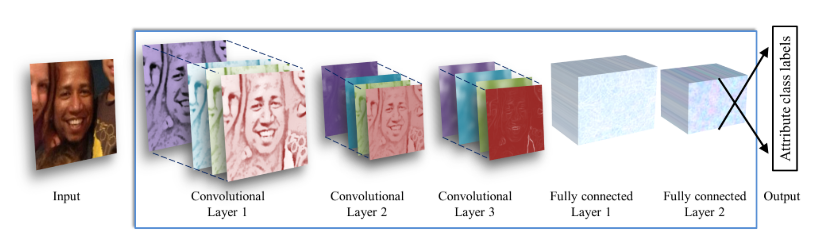
\includegraphics[width=\textwidth]{figure_2.png}
与例如[18]中用于训练用于面部识别的网络的一万个身份等级相比较,我们选择较小的网络设计,这源于我们希望降低过度拟合的风险以及我们试图解决的问题的性质:Adience集合上的年龄分类需要区分八个类别,而性别只有两个。\\
所有三个颜色通道都由网络直接处理。首先将图像重新缩放为256×256,并将227×227的作物馈送到网络。然后如下定义三个随后的卷积层。\\
\textbf{1.}将尺寸为3×7×7像素的96个滤波器应用于第一卷积层的输入,然后是整流线性算子(ReLU),最大池值采用2像素的3×3区域的最大值步幅和局部响应归一化层。\\
\textbf{2.}然后由第二卷积层处理前一层的96×28×28输出,包含256个大小为96×5×5像素的滤波器。同样,接下来是ReLU,一个最大池化层和一个本地响应归一化层,具有与以前相同的超参数。\\
\textbf{3.}最后,通过应用一组尺寸为256×3×3像素的384个滤波器,然后是ReLU和最大汇集层,第三个和最后一个卷积层在256×14×14点上操作。\\\\
然后通过以下定义以下全连接层:\\\\
\textbf{4.}第一个全连接层,其接收第三卷积层的输出并包含512个神经元,接着是ReLU和丢失层。\\
\textbf{5.}第二全连接层,其接收第一全连接层的512维输出​​并且再次包含512个神经元,接着是ReLU和丢失层。\\
\textbf{6.}第三个全连接的层,映射到年龄或性别的最终类。\\
最后,最后一个全连接层的输出被馈送到soft-max层,该层为每个类分配概率。预测本身是通过对给定测试图像采用具有最大概率的类来进行的。\\

\subsection{测试与训练}
\textbf{初始化}
所有层中的权重用来自零均值高斯的随机值初始化,标准偏差为0.01。
为了强调这一点,我们不使用预先训练的模型来初始化网络;网络是从头开始训练的,不使用图像之外的任何数据和基准测试可用的标签。\\
训练的目标值表示为对应于基础真值类的稀疏二元向量。对于每个训练图像,目标标签向量是类别数量的长度(两个用于性别,八个用于年龄分类任务),在地面实况的索引中包含1,在其他地方包含0。\\

\textbf{网络训练}
除了我们使用精简网络架构外,我们还应用了另外两种方法来进一步限制过度拟合的风险。
首先,我们应用Drop-out learning(即随机将网络神经元的输出值设置为零)。该网络包括两个丢失层,其丢失率为0.5(将神经元输出值设置为零的几率为50%)。
其次,我们通过从256×256输入图像中随机选区227×227像素并在每个前后训练传递中随机镜像来使用数据增强。\\

训练本身使用随机梯度进行,图像批量大小为50个图像。初始学习率为$e^-3$,在10K迭代后减少到$e^-4$。\\

\textbf{预测}
我们尝试了两种使用网络的方法,以便为新数据制作年龄和性别预测:\\
\begin{itemize}
    \item \textbf{中心裁剪} :使用脸部图像回馈网络,在脸部中心周围裁剪为227×227。\\
    \item \textbf{过采样} :我们从256×256面部图像的角落中提取五个227×227像素裁剪区域,从面部中心提取另外的裁剪区域。网络呈现所有五个图像,以及它们的水平反射。其最终预测被视为所有这些变化的平均预测值。\\
\end{itemize}

我们发现,由于这些图像的许多挑战(像素,运动模糊等)导致的Adience图像中的小错位会对结果的质量产生显着影响。
第二种过采样方法旨在弥补这些小的错位,避免了改善对齐质量的需要,而是直接向网络提供同一面的多个转换版本。\\

\section{实验}
我们的方法是使用Caffe开源框架实现的。在拥有1,536个CUDA核心和4GB视频内存的GPU机器上进行了培训。训练每个网络需要大约四个小时,使用我们的网络预测单个图像上的年龄或性别需要大约200ms。
通过在图像批次上运行网络,可以显着改善预测运行时间。\\

\subsection{Adience基准}
我们使用最近发布的Adience基准测试了CNN设计的准确性,该基准用于年龄和性别分类。
Adience集包含从智能手机设备自动上传到Flickr的图像。因为这些图像是在没有事先手动过滤的情况下上传的,例如媒体网页上的情况(例如,来自LFW集合的图像)或社交网站,这些图像的质量高度不受约束,反映了互联网图像中出现的许多面孔现实挑战。\\

\subsection{结果}

表1和表2分别给出了性别和年龄分类的结果。
表3进一步提供了我们的多类年龄分类结果的混淆矩阵。对于年龄分类,我们测量并比较算法给出精确年龄组分类时的准确度和算法何时不起作用。
这反映了任务固有的不确定性,即面部特征在一个年龄阶段的最老面孔和后续阶层中最年轻的面孔之间经常变化很小。\\

显然,所提出的方法在两个任务中都具有相当大的成果,优于所报告的最新技术水平。
同样明显的是过采样方法的贡献,它提供了比原始网络更多的性能提升。这意味着更好的规则图像可以提供额外的性能提升。\\

我们分别在图4和图5中提供了一些性别和年龄错误分类的例子。这些表明我们的系统所犯的许多错误都是由于某些基准测试图像的观察条件非常具有挑战性。
最值得注意的是由模糊或低分辨率和遮挡(尤其是浓妆)引起的错误。对于尚未看到明显性别属性的婴儿或幼儿的图像,经常会出现性别估计错误\\
\section{结论}
虽然许多以前的方法已经解决了年龄和性别分类的问题,但直到最近,这项工作的大部分都集中在实验室环境中拍摄的受限图像上。这些设置不能充分反映社交网站和在线存储库中真实图像的常见变化。
然而,互联网图像不仅具有更大的挑战性:它们也是不可或缺的。大型图像集的轻松可用性为现代机器学习系统提供了有效无限的训练数据,尽管这些数据并不总是适合监督学习。\\

以相关的人脸识别问题为例,我们探讨了CNN在使用互联网数据的情况下对这些任务的执行情况。
我们通过精益深度学习架构提供结果,旨在避免由于有限标签数据的限制而过度拟合。
与一些最近的网络架构相比,我们的网络较小,从而减少了参数数量和过度拟合的可能性。
我们通过人工添加训练集中的图像裁剪版本来进一步扩大训练数据的大小,得到的结果在未经过滤的图像的Adience基准测试中显示出优于最新技术水平的结果。\\

从我们的结果中可以得出两个重要结论。
首先,CNN可用于提供改进的年龄和性别分类结果,甚至考虑到当前无约束图像集的尺寸很小的年龄和性别标记。
其次,我们模型的简单性表明,使用更多训练数据的更复杂的系统可能能够大大改善结果,而不是这里报告的结果。\\
\end{document}